\section{Logical View}
Die logische Sicht beschreibt die Funktionalität der Komponenten. Dazu wird ein UML-Klassendiagramm für jeden 
Microservice bereitgestellt. Um die Lesbarkeit zu verbessern, werden die Bibliotheksklassen von \textit{spring} und \textit{fastify} nicht in den Diagrammen dargestellt.
Zusätzlich sind der Entity- und der Tracking-Service in einem nicht OOP-Stil in Typescript entwickelt worden. Da sie keine Klassen haben, basieren ihre Klassendiagramme nicht auf Klassen, sondern auf deren Module. Dadurch können die Funktionalitäten ähnlich zu einem klassichen Klassendiagramm abgebildet werden.

\subsection{Entity-Service}
\begin{figure}[!ht]
    \centering
    \makebox[0pt]{%
    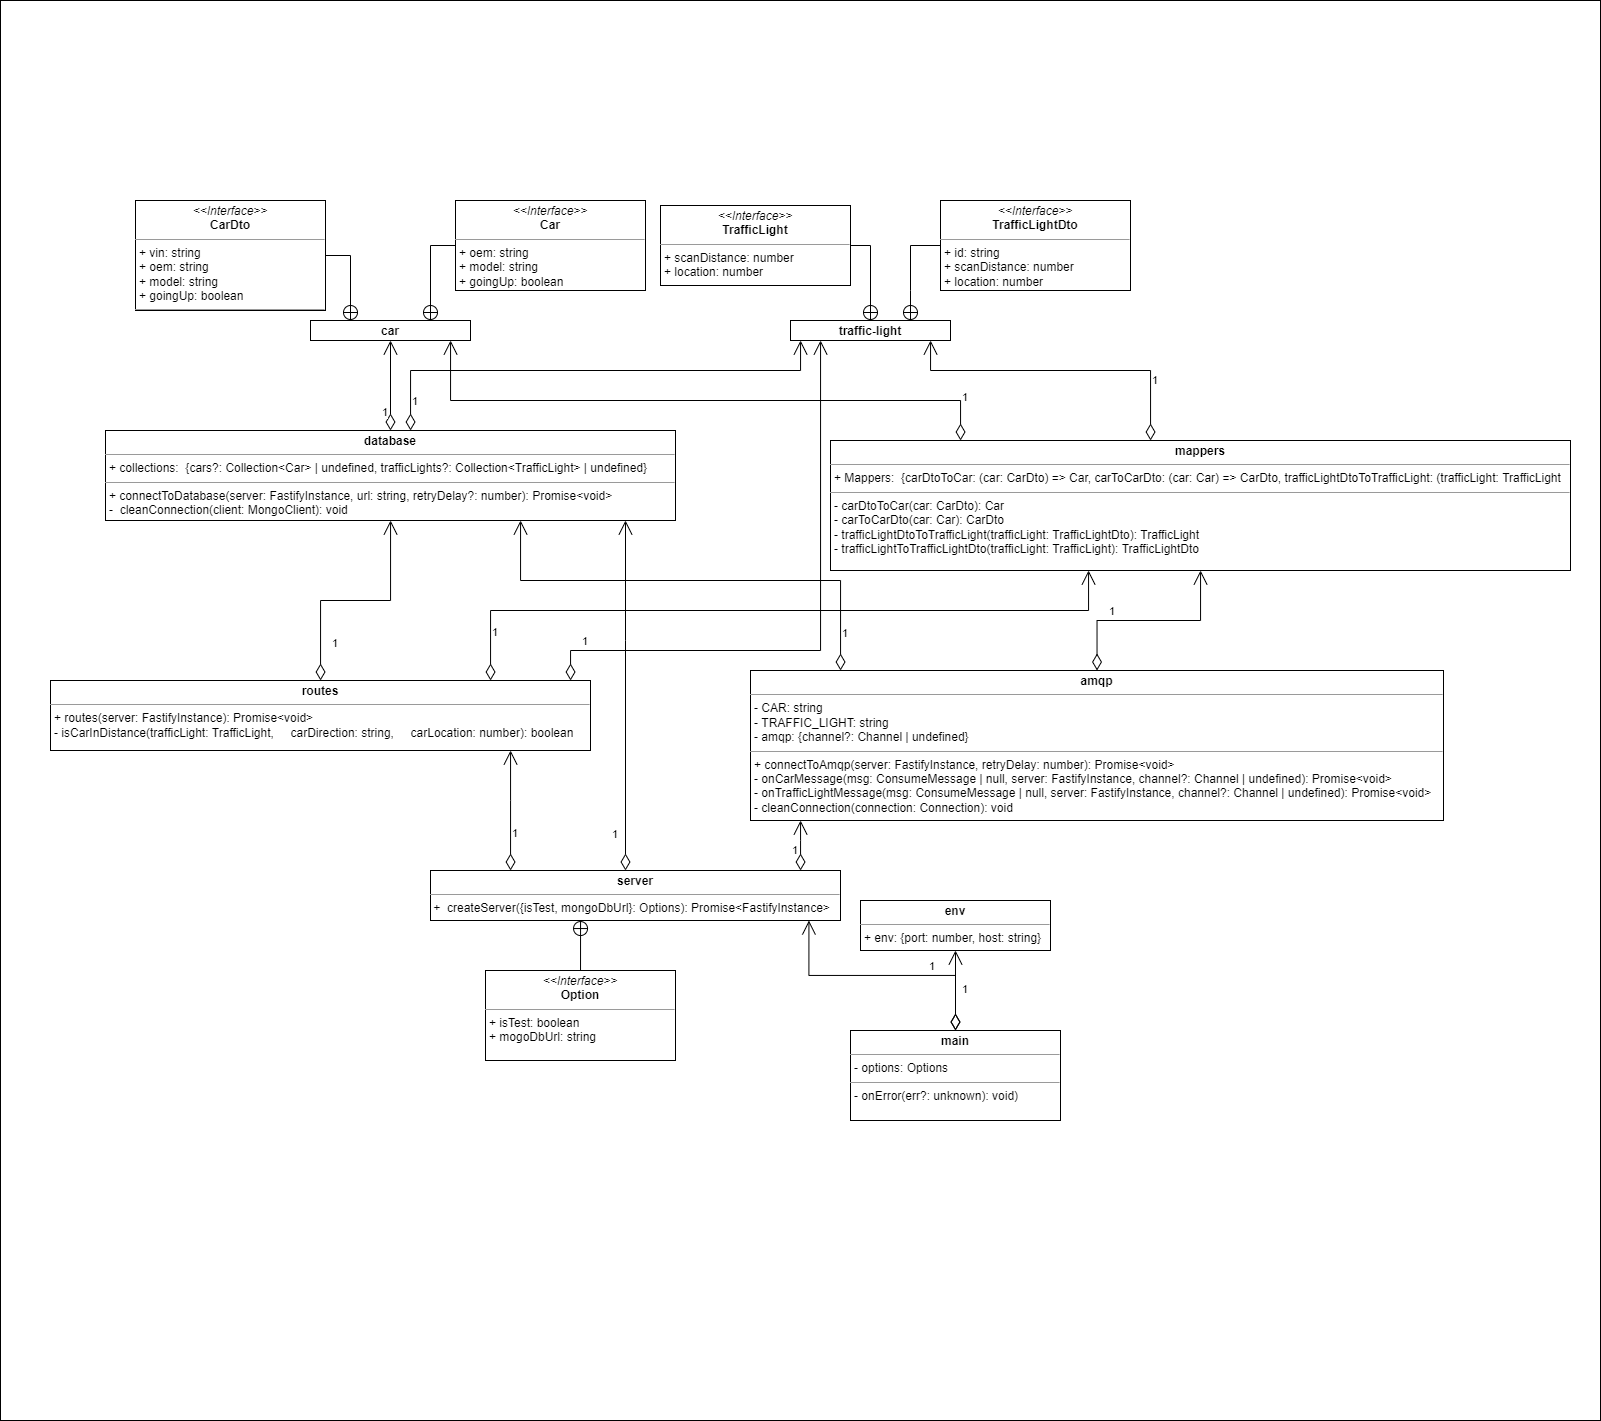
\includegraphics[width=18cm]{./figure/entity-service-uml.png}}
    \caption{Entity-Service UML}
    \label{fig:entity-service}
\end{figure}
\subsection{Tracking-Service}
\begin{figure}[!ht]
    \centering
    \makebox[0pt]{%
    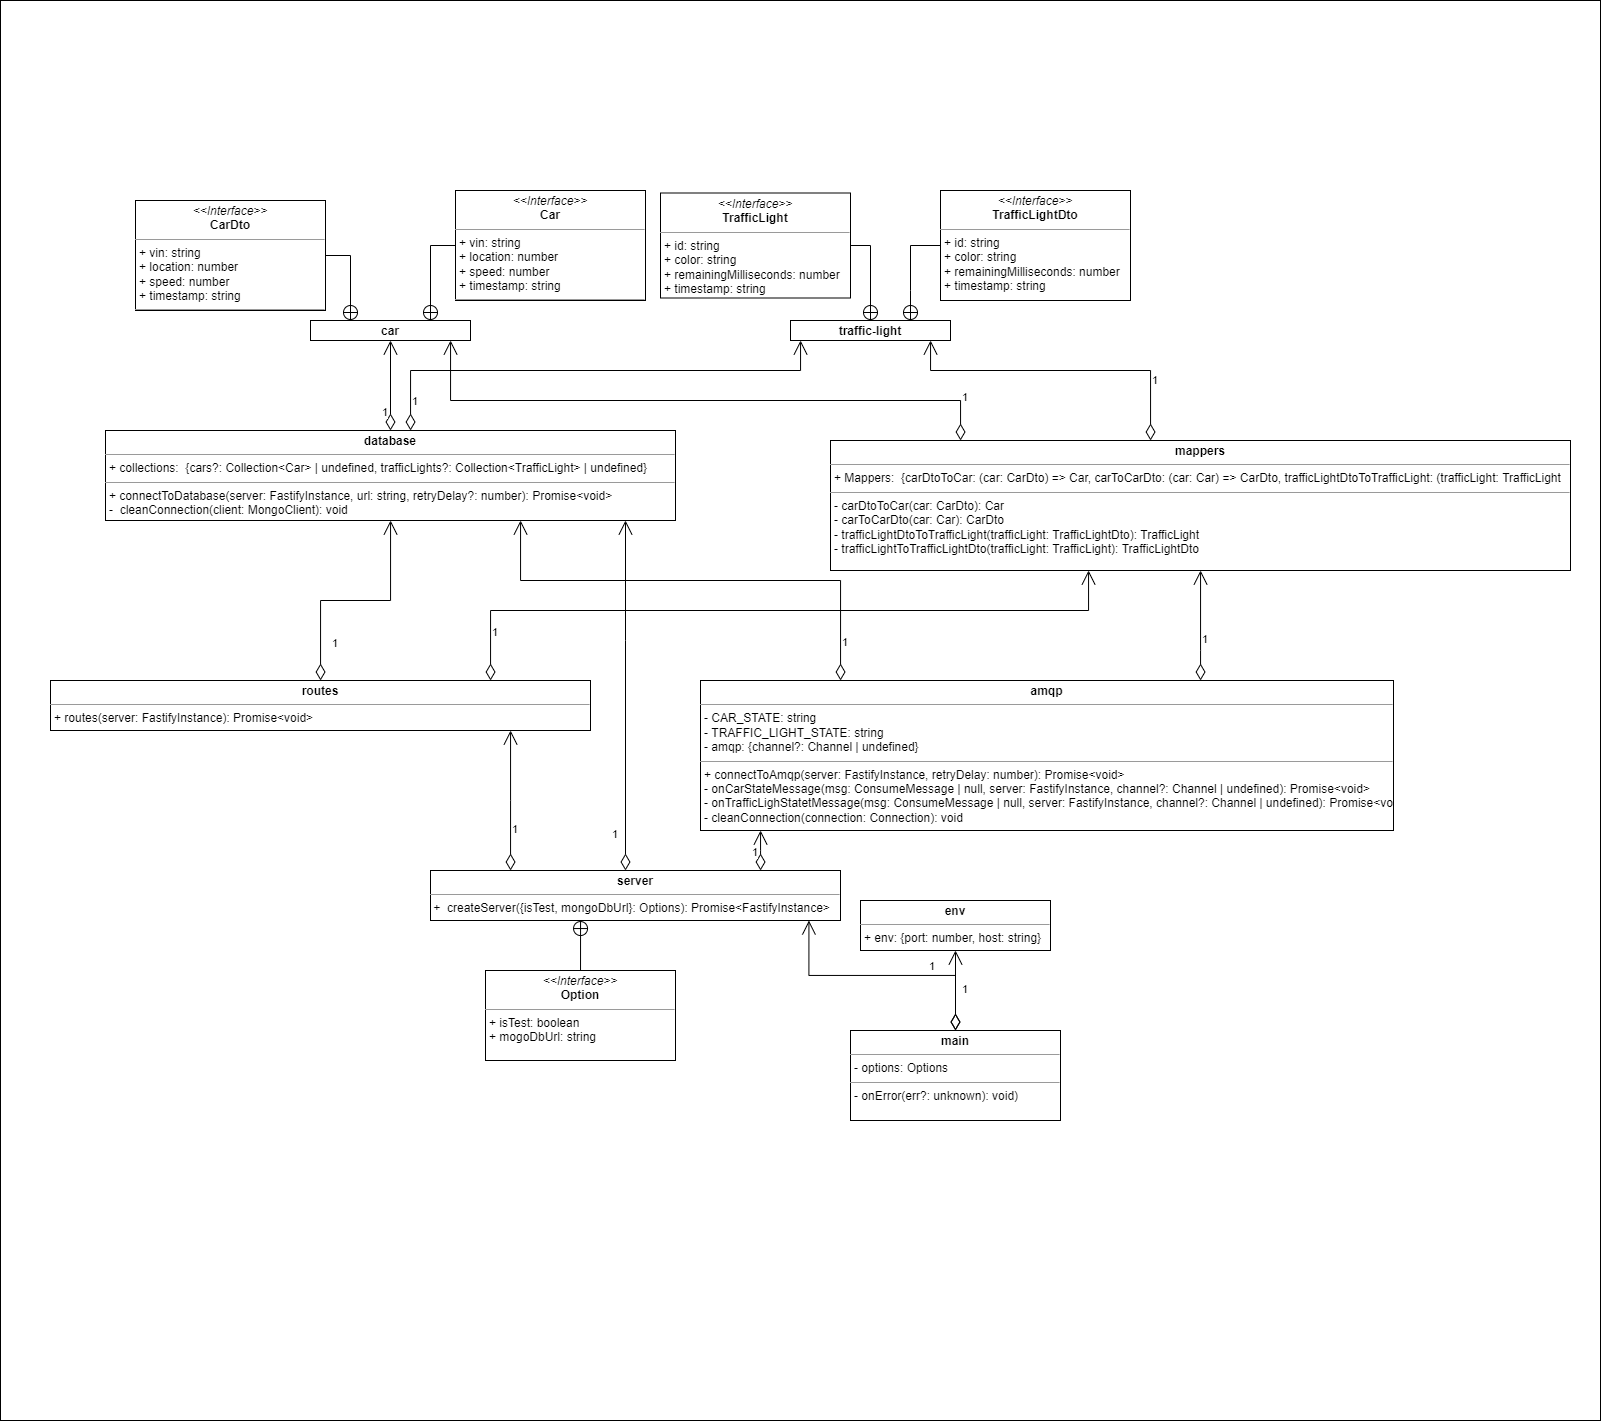
\includegraphics[width=18cm]{./figure/tracking-service.png}}
    \caption{Tracking-Service UML}
    \label{fig:tracking-service}
\end{figure}
